%
% HSR LaTex Template
% Copyright 2012, Florian Bentele
%
% Complete LaTex template for thesis at HSR, customized
% for Prof. Dr. Peter Heinzmann
%
%
% This document is free software: you can redistribute
% it and/or modify it under the terms of the GNU
% General Public License as published by the Free
% Software Foundation, either version 3 of the License,
% or (at your option) any later version.
%
% This document is distributed in the hope that it will
% be useful, but WITHOUT ANY WARRANTY; without even the
% implied warranty of MERCHANTABILITY or FITNESS FOR A
% PARTICULAR PURPOSE. See the GNU General Public1
% License for more details.1
%
% You should have received a copy of the GNU General
% Public License along with this document. If not, see
% <http://www.gnu.org/licenses/>.
%

\documentclass[11pt,twoside]{hsrthesis}

%\makeindex

% do this here, so you can \gls{...} to it
%%add new glossaryentries here...

\newglossaryentry{sqlite}{
	name=SQLite,
	description={SQLite ist eine Datenbankengine, welche ohne Konfiguration auskommt. Es handelt sich dabei um eine Datenbank in einer Datei},
	first={SQLite}
}
%\makeglossaries

\begin{document}

\newcommand{\thesistitle}{Teamreview 2}
\newcommand{\thesisauthora}{Pascal Horat, Steve Gerome Kamga, Gökhan Kaya}
\newcommand{\thesisauthorb}{}
\newcommand{\thesisauthorc}{}
\newcommand{\professor}{Prof. Dr. Some Body}
\newcommand{\thesistype}{Bachelorarbeit}
\newcommand{\departement}{Abteilung Informatik}
\newcommand{\school}{Hochschule für Technik Rapperswil}
\newcommand{\term}{Frühjahrssemester 2017}
\newcommand{\thedate}{21. März 2017}
\newcommand{\timeperiode}{21.02.2012 - 01.06.2012}
\newcommand{\partner}{-}
\newcommand{\workload}{-}
\newcommand{\linktothesis}{https://moodle.hsr.ch}

\setlength{\oddsidemargin}{20mm}
\maketitle
\setlength{\oddsidemargin}{20mm}


\tableofcontents


% The main content
%%%%%%%%%%%%%%%%%%
%\begin{comment}
\chapter*{Examples}

\section*{Glossary Example}

\gls{sqlite} ist ein Glossar Eintrag. Lorem ipsum dolor sit amet, consetetur sadipscing elitr, sed diam nonumy eirmod tempor invidunt ut labore et dolore magna aliquyam erat, sed diam voluptua. At vero eos et accusam et justo duo dolores et ea rebum.

\section*{Bibliography and Citation Example}

Dies ist ein Zitat aus einem Buch\cite{Matthews201111}. Lorem ipsum dolor sit amet, consetetur sadipscing elitr, sed diam nonumy eirmod tempor invidunt ut labore et dolore magna aliquyam erat, sed diam voluptua. At vero eos et accusam et justo duo dolores et ea rebum.

Lorem ipsum dolor sit amet, consetetur sadipscing elitr, sed diam nonumy eirmod tempor invidunt ut labore et dolore magna aliquyam erat, sed diam voluptua. At vero eos et accusam et justo duo dolores et ea rebum. Stet clita kasd gubergren, no sea takimata sanctus est Lorem ipsum dolor sit amet. Lorem ipsum dolor sit amet, consetetur sadipscing elitr, sed diam nonumy eirmod tempor invidunt ut labore et dolore magna aliquyam erat, sed diam voluptua. At vero eos et accusam et justo duo dolores et ea rebum. Stet clita kasd gubergren, no sea takimata sanctus est Lorem ipsum dolor sit amet. Lorem ipsum dolor sit amet, consetetur sadipscing elitr, sed diam nonumy eirmod tempor invidunt ut labore et dolore magna aliquyam erat, sed diam voluptua. At vero eos et accusam et justo duo dolores et ea rebum. Stet clita kasd gubergren, no sea takimata sanctus est Lorem ipsum dolor sit amet. 

Duis autem vel eum iriure dolor in hendrerit in vulputate velit esse molestie consequat, vel illum dolore eu feugiat nulla facilisis at vero eros et accumsan et iusto odio dignissim qui blandit praesent luptatum zzril delenit augue duis dolore te feugait nulla facilisi. Lorem ipsum dolor sit amet, consectetuer adipiscing elit, sed diam nonummy nibh euismod tincidunt ut laoreet dolore magna aliquam erat volutpat. 

Ut wisi enim ad minim veniam, quis nostrud exerci tation ullamcorper suscipit lobortis nisl ut aliquip ex ea commodo consequat. Duis autem vel eum iriure dolor in hendrerit in vulputate velit esse molestie consequat, vel illum dolore eu feugiat nulla facilisis at vero eros et accumsan et iusto odio dignissim qui blandit praesent luptatum zzril delenit augue duis dolore te feugait nulla facilisi. 


\section*{Table Examples}
\subsection*{Automagical Column Widths}
\begin{tabularx}{\textwidth}{X X X X} \beforeheading
\heading{Heading 1} & \heading{Heading 2} & \heading{Heading 3} & \heading{Heading 4} \\\afterheading
Cell 1,1 & Cell 1,2 & Cell 1,3 & Cell 1,4 \\\normalline
Cell 2,1 & Cell 2,2 & Cell 2,3 Vel illum dolore eu feugiat nulla facilisis at vero eros et accumsan et iusto odio dignissim qui blandit praesent luptatum zzril delenit augue duis dolore te feugait nulla facilisi. & Cell 2,4 \\\normalline
Cell 3,1 Duis autem vel eum iriure dolor in hendrerit in vulputate velit esse molestie consequat. & Cell 3,2 & Cell 3,3 & Cell 3,4 \\\lastline
\end{tabularx}

\subsection*{Column Alignment \& Filler}
\begin{tabularx}{\textwidth}{l c r X} \beforeheading
\heading{Left Aligned} & \heading{Centered} & \heading{Right Aligned} & \heading{Filler} \\\afterheading
Cell 1,1 & Cell 1,2 & Cell 1,3 & Cell 1,4 Ut wisi enim ad minim veniam, quis nostrud exerci tation ullamcorper  \\\normalline
Cell 2,1 & Cell 2,2 & Cell 2,3 & Cell 2,4 Ut wisi enim ad minim veniam, quis nostrud exerci tation ullamcorper  \\\normalline
Cell 3,1 & Cell 3,2 & Cell 3,3 & Cell 3,4 Ut wisi enim ad minim veniam, quis nostrud exerci tation ullamcorper  \\\lastline
\end{tabularx}
\end{comment}
%03introduction.tex

\chapter{Ziel dieses Dokumentes}

Das Ziel dieses Dokuments ist es, die im HSR-Modul Teamkommunikation für Ingenieure erlernten Teamrollen-Modelle anwenden zu können und diese den Teammitgliedern zuzuordnen. So sollen potenzielle Stärken und Schwächen des Teams entdeckt und Konsequenzen eingeleitet werden. 


\makeatletter				%Damit kein pagebreak bei neuem chapter
\patchcmd{\chapter}{\if@openright\cleardoublepage\else\clearpage\fi}{}{}{} 
%Damit kein pagebreak bei neuem chapter
\makeatother				%Damit kein pagebreak bei neuem chapter
%04chapterSelbsteinsch.tex
\chapter{Individuelle Teameinschätzung}

Anhand folgender Tabellen ist ersichtlich, zu welchem Grad die Mitglieder unseres Teams die verschiedenen Ausprägungen der Teameffektivität \cite{Simon3} eingeschätzt haben.

\begin{figure}[!h]
  \centering
    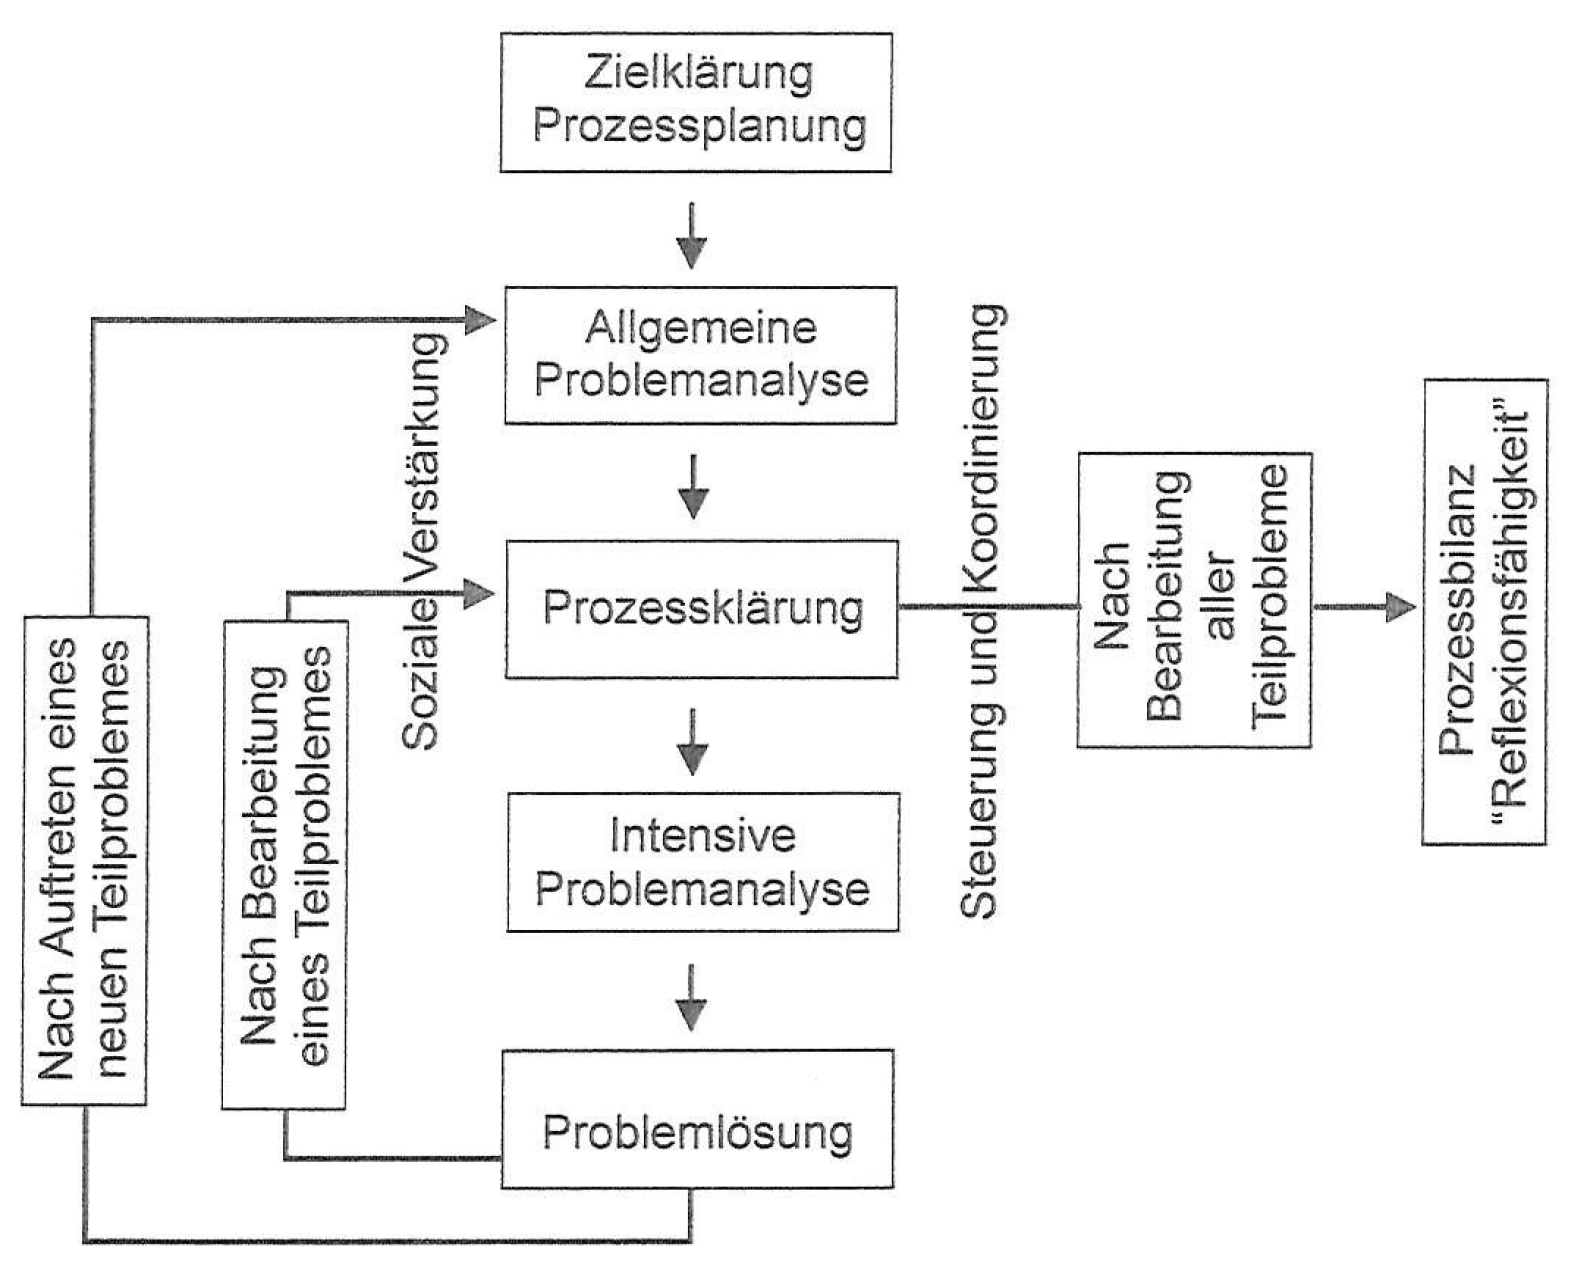
\includegraphics[height=10cm]{images/optimalerProblemloeseverlauf.png}
  \caption{optimaler Problemlöseverlauf}
  \label{fig:problem}
\end{figure}

\newcommand{\abstand}{0.7cm}
\newcommand{\fabstand}{1.2cm}
\newcolumntype{C}[1]{>{\centering\arraybackslash}p{#1}} % zentriert mit Breitenangabe

\subsection*{Gökhan}
\begin{tabular}{C{\fabstand}|C{\abstand}|C{\abstand}|C{\abstand}|C{\abstand}|C{\abstand}|C{\abstand}|C{\abstand}|C{\abstand}|C{\abstand}|C{\abstand}|C{\abstand}|}
\hline
& -5 & -4 & -3 & -2 & -1 & 0 & +1 & +2 & +3 & +4 & +5\\
\hline
&\begin{tiny}nicht vorhanden \end{tiny}& & & & & \begin{tiny}genau richtig \end{tiny}& & & & & \begin{tiny}viel zu ausgeprägt\end{tiny}\\
\hline
\begin{tiny} Reflexions-fähigkeit \end{tiny} & & & & & & x & & & & & \\
\hline
\begin{tiny} Prozessklärungs-fähigkeit \end{tiny}& & & & & x & & & & & & \\
\hline
\begin{tiny} Koordinations-fähigkeit \end{tiny}& & & & & x & & & & & & \\
\hline
\begin{tiny} Entscheidungs-fähigkeit \end{tiny}& & & & & & & x & & & & \\
\hline
\begin{tiny} Soziale Unterstützung \end{tiny}& & & & & & x & & & & & \\
\hline
\end{tabular}

\subsection*{Gerome}

\begin{tabular}{C{\fabstand}|C{\abstand}|C{\abstand}|C{\abstand}|C{\abstand}|C{\abstand}|C{\abstand}|C{\abstand}|C{\abstand}|C{\abstand}|C{\abstand}|C{\abstand}|}
\hline
& -5 & -4 & -3 & -2 & -1 & 0 & +1 & +2 & +3 & +4 & +5\\
\hline
&\begin{tiny}nicht vorhanden \end{tiny}& & & & & \begin{tiny}genau richtig \end{tiny}& & & & & \begin{tiny}viel zu ausgeprägt\end{tiny}\\
\hline
\begin{tiny} Reflexions-fähigkeit \end{tiny} & & & & & & & & x & & & \\
\hline
\begin{tiny} Prozessklärungs-fähigkeit \end{tiny}& & & & & & & & x & & & \\
\hline
\begin{tiny} Koordinations-fähigkeit \end{tiny}& & & & & & & x & & & & \\
\hline
\begin{tiny} Entscheidungs-fähigkeit \end{tiny}& & & & & & & x & & & & \\
\hline
\begin{tiny} Soziale Unterstützung \end{tiny}& & & & & & x & & & & & \\
\hline
\end{tabular}

\subsection*{Pascal}

\begin{tabular}{C{\fabstand}|C{\abstand}|C{\abstand}|C{\abstand}|C{\abstand}|C{\abstand}|C{\abstand}|C{\abstand}|C{\abstand}|C{\abstand}|C{\abstand}|C{\abstand}|}
\hline
& -5 & -4 & -3 & -2 & -1 & 0 & +1 & +2 & +3 & +4 & +5\\
\hline
&\begin{tiny}nicht vorhanden \end{tiny}& & & & & \begin{tiny}genau richtig \end{tiny}& & & & & \begin{tiny}viel zu ausgeprägt\end{tiny}\\
\hline
\begin{tiny} Reflexions-fähigkeit \end{tiny} & & & & & x & & & & & & \\
\hline
\begin{tiny} Prozessklärungs-fähigkeit \end{tiny}& & & & x & & & & & & & \\
\hline
\begin{tiny} Koordinations-fähigkeit \end{tiny}& & & & x & & & & & & & \\
\hline
\begin{tiny} Entscheidungs-fähigkeit \end{tiny}& & & & & x & & & & & & \\
\hline
\begin{tiny} Soziale Unterstützung \end{tiny}& & & & & & & x & & & & \\
\hline
\end{tabular}\\

Auf dem Spiderwebchart \ref{fig:web} sind die Daten aus obigen Tabellen grafisch noch einmal dargestellt. An den Ecken des Pentagons sind die verschiedenen Bereiche der Teameffektivität \cite{Simon1} verteilt. Die Farben zeigen die drei Teammitglieder. Die Ausprägung kann anhand der Werteskala (im Zentrum minus 5 und an den Ecken plus 5 abgelesen werden).
Ein Vergleich zeigt, dass Gökhan und Pascal eine ziemlich ähnliche Einschätzung haben, wobei Gerome eher höhere Werte gewählt hat und daher er die verschiedenen Bereiche als ausgeprägter auffasst.

\begin{figure}[!h]
  \centering
    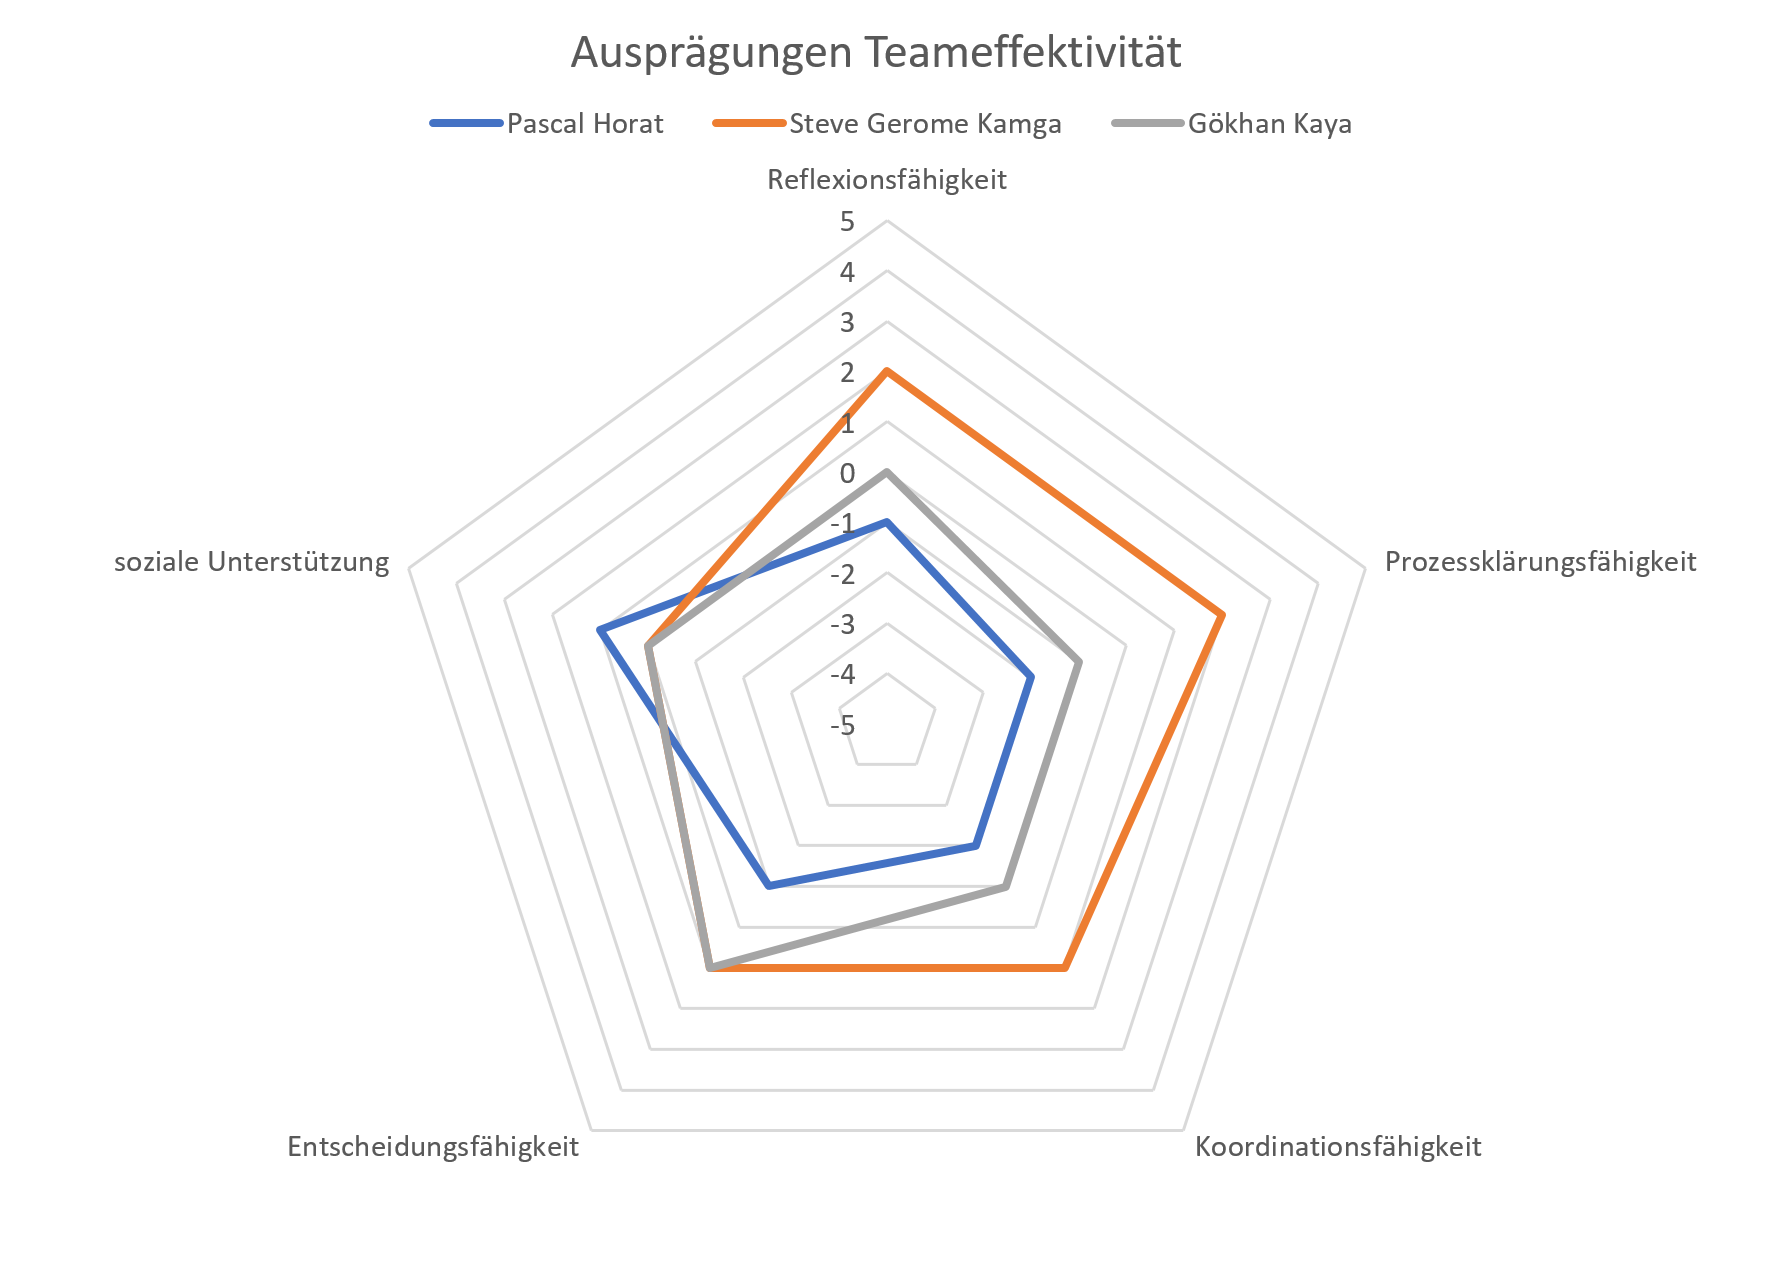
\includegraphics[height=11cm]{images/AuspraegungenTeameffektivitaet.png}
  \caption{Ausprägungen der Teameffektivität}
  \label{fig:web}
\end{figure}

\begin{comment}
In diesem Kapitel wird beschrieben, welche Rollen die Teammitglieder mittels Selbsteinsch"atzung erhalten. Dazu wird ein Test verwendet, welcher urspr"unglich von R.M. Belbin \cite{belbin1981management} entwickelt und an der Universit"at Regensburg ins Deutsche übersetzt wurde\cite{Studienbrief}. In diesem Test werden verschiedenste Aussagen bezüglich des eigenen Verhaltens in bestimmten Situationen mittels eines Punktesystems bewertet. Am Ende trägt man die Punkte in ein Raster ein, aus welchem sich dann die passenden Rollen herauskristallisieren.

\subsection*{Pascal Horat}
Da ich in meinem Leben schon andere, ähnliche Tests ausgefüllt habe, wusste ich welche Rollen ich als Resultat in etwa zu erwarten hatte. Trotzdem war ich gespannt, ob sich auch dieses Mal dieselben Tendenzen zeigen würden. \\

Tatsächlich erreichte, wie von mir im vornherein erwartet, die Rolle des Koordinators die höchste Punktzahl. Allerdings war ich überrascht mit welcher Deutlichkeit das Resultat ausfiel. Wie in obiger Grafik ersichtlich, haben die Rolle des Pragmatikers und des Vollenders die zweitgrösste Ausprägung (orange markiert). Auch sieht man, das die Visionärsrolle und die des Akquisiteurs fast keine Punkte erhalten haben. Die äusserst niedrige Punkteausbeute beim Visionär hat mich eher überrascht. Ich finde nämlich, das oft alternative Ansätze und neue Ideen von meiner Seite kommen.

\subsection*{Steve Gerome Kamga}
Das Resultat meiner Auswertung mit der Belbin-Methode hat einige Teamrollen aufgezeigt, die zu meinen Fähigkeiten und meinem Verhalten bezüglich der Zusammenarbeit passen könnten. Nachfolgend werden die drei Teamrollen erwähnt, bei denen ich die meisten Punkte bekommen habe.
Als erstes kommt der Pragmatiker, der sich als eine auf die anstehende Sache und entsprechendes praktisches Handeln gerichtete Person definieren lässt. Danach folgen der Spezialist und der Vollender.
\newline
Nach dieser Bewertungsmethode habe ich in Ruhe die drei obengenannten Teamrollen überdacht und mir einige persönliche Fragen gestellt. Resultierend würde ich sagen, dass die Ergebnisse bei mir mindestens zu 60\% stimmen, obwohl die Belbin-Methode nur auf Einschätzungen basiert.


\subsection*{Gökhan Kaya}

Meine Auswertung der Selbsteinschätzung gemäss Belbin ergab die folgende Punkteverteilung:

\begin{tabular}{lr}
  Visionär & 2 \\ 
  Akquisiteur & 5 \\ 
  Prozessgestalter & 8 \\ 
  Koordinator & 10 \\ 
  Bewerter & 2 \\
  Ausgleicher & 19 \\
  Pragmatiker & 7 \\
  Vollender & 6 \\
  Spezialist & 11 \\
\end{tabular}
\newline


Somit ist zu sehen, dass folgende drei Teamrollen herausstechen:
%\renewcommand{\labelenumi}{\roman{enumi}} 
\begin{enumerate} 
\item Ausgleicher 
\item Spezialist
\item Koordinator
\end{enumerate}

Wobei besonders die Rolle des Ausgleichers mit 19 Punkten hervorsticht. Dies war für mich keine Überraschung, da sich während den Teamsitzungen bereits herauskristallisierte, dass der gute Teamzusammenhalt einer meiner Hauptziele geworden war. Ich habe mich entsprechend eingesetzt und immer wieder versucht herauszufinden, ob alle mit den getroffenen Entscheidungen zufrieden waren und wirklich nichts auszusetzen hatten. Falls doch habe ich versucht, mir die Meinung jedes einzelnen anzuhören und auszudiskutieren.
\end{comment}


%04chapterFremdeinsch.tex
\chapter{Gruppeneinschätzung des Teams}\label{Gruppenteameinschätzung}

Als Anregung unserer Diskussion zur Gruppeneinschätzung und damit wir einen Leitfaden haben, verwenden wir das Dokument Leitfragen für Team-Selbsteinschätzung (REFERENZ EINFÜGEN). Aus diesem Dokument haben wir folgende Fragen kopiert, welche wir nun beantworten werden.
  
\subsection*{Wie diskutieren die Teammitglieder Probleme?}

Die Mehrheit der Gruppe findet, dass die Probleme offen angesprochen werden. Jedoch findet Pascal, dass Probleme viel öfter zur Sprache gebracht werden und konstruktive Kritik an der Tagesordnung sein sollte. 
Probleme wurden Anfangs nur in Sitzungen angesprochen. Dies wollen wir ändern und zu einem laufenden Prozess machen. 

\subsection*{Wie gehen Teammitglieder mit Defiziten und unproduktiven Verhaltensweisen um?}

Anfangs waren die Arbeitszeiten sehr hoch. Dies wurde im Team schnell so zur Diskussion gebracht und Verbesserungsvorschläge unterbreitet. Nach einigen Diskussionen haben wir einiges an unserem Vorgehen angepasst und hoffen nun auf eine Effizienzsteigerung. Daher glauben wir, dass wir mit Defiziten und unproduktiven Verhaltensweisen sehr offen umgehen.

\subsection*{Was wissen Sie darüber, was Ihre Kollegen gerade machen und was Sie zum
Gruppenziel beitragen?}

Aufträge wurden jeweils am Anfang der Vorlesung jede Woche neu verteilt. In der Zwischenzeit war oft nicht klar, wer was bereits erledigt hat. Durch vermehrte Nutzung von MS-Project, erhöhtem Koordinationsaufwand (Aufträge in kürzeren Abständen) und einer klar definierten Führung, erhoffen wir uns mit weniger zeitlichem Aufwand bessere Produkte erstellen zu können.

\subsection*{Wie verhalten sich Teammitglieder, wenn sie etwas Unpassendes oder möglicherweise Teamschädliches gesagt oder getan haben?}

Keiner der Teammitglieder hatte bisher das Gefühl, teamschädigenden oder unpassenden Aussagen ausgesetzt zu sein.

\subsection*{Wie gehen Sie mit Wissensunterschieden im Team um?}

Das Wissen in unserem Team war und ist sehr unterschiedlich verteilt. 
In der Regel werden die Wissensunterschiede im Team gemeinsam ausgeglichen oder es wird erwartet, dass sich die Person selbstständig informiert. Als konkretes Beispiel ist zu erwähnen, dass am Anfang Gökhan bereits latex und Git Erfahrung hatte, während sich die anderen Teammitglieder noch nicht mit mit diesen Medien auseinandergesetzt hatten. Pascal und Gökhan haben sich selbstständig und ohne weitere Hilfe mit den neuen Medien auseinandersetzten, wobei dies bei Gerome teilweise nicht möglich war, da unter anderem ein entsprechend ausgestatteter Computer fehlte. Der dabei entstandene Wissensunterschied wird momentan in der Gruppe gemeinsam aufgeholt und gleichzeitig erwartet, dass sich Gerome selbstständig weiterbildet.  

\subsection*{Wie würden Sie Ihr Teamverhalten gegenüber Aussenstehenden (andere Abteilungen,
Kunden, Lieferanten) beschreiben?}

Der einzige Kontakt gegenüber Aussenstehenden ist der Dozent. Dieser ist zufriedenstellend. 

\subsection*{Wie zeigen Teammitglieder Engagement? Woran erkennen Sie (fehlendes)
Engagement?}

Das Teamengagement der Teammitglieder kann durch diverse Verhaltensweisen erkannt werden. Nachfolgend listen wir einige wichtige Erkennungsmerkmale auf.

\begin{itemize}

\item Freiwilliges Übernehmen von kleineren ausstehenden Arbeiten

\item Bereitschaft länger zu arbeiten, als dies zwingend nötig wäre

\item Beteiligung an Diskussionen

\item Pünktlichkeit

\end{itemize}

Bei Pascal ist zu erkennen, dass er oft kleinere anstehende Arbeiten freiwillig übernimmt und nicht zwingend notwendige arbeiten erledigt, damit das Projekt einem noch höheren Standard gerecht wird. 

Gökhan nimmt sich bei technischen Schwierigkeiten gerne für jeden Zeit und beteiligt sich ausserdem konstruktiv an Gesprächen.  

Gerome beteiligt sich ebenfalls gerne und konstruktiv an Gesprächen. Er hat eine ausserordentlichen Bereitschaft, längere Arbeitssessionen mit der Gruppe zu führen und dabei immer gut gelaunt zu bleiben. Die Pünktlichkeit lässt jedoch etwas zu wünschen übrig.  

\subsection*{Wie würden Sie Ihre Teamsitzungen beschreiben? Welchen Beitrag leisten diese zum
Teamerfolg?}

Der hauptsächliche Mehrwert, der in den bisherigen Sitzungen generiert wurde, war der Wissensausgleich der einzelnen Teammitglieder. Vor allem anfangs wurde aber noch zu wenige konkrete Handlungen aus diesen Sitzungen abgeleitet. 

\subsection*{Wie verhalten Sie sich, wenn Sie merken, dass die Gruppenziele (möglicherweise)
nicht erreicht werden können?}

Als wir den Gesammtumfang des AC-Produktes das erste mal vor Augen hatten, wurde uns bewusst, dass wir dieses nur mit einer neuen Strategie, bei welcher eine Person eine erhöhte koordinierende Rolle einnimmt bewältigt werden kann. 

\subsection*{Was wissen Sie über das Privatleben der anderen Teammitglieder?}

Während den gemeinsam erledigten Arbeiten konnten wir uns bereits privat etwas besser kennenlernen, indem wir beispielsweise gemeinsam gekocht haben, als wir längere Arbeiten verrichten mussten. 

\subsection*{Wie treffen Sie Entscheidungen im Team?}

Wie in unserem Regeldokument beschlossen, wurden Entscheidungen bisher nach dem Prinzip des Mehrheitsentscheides gefällt.

\subsection*{Was tun Sie, wenn Sie mit einer Entscheidung nicht einverstanden sind?}

Die Diskrepanz wird zur Sprache gebracht und anschliessend demokratisch entschieden.

\subsection*{Wie gehen Sie mit Lob und Kritik im Team um?}

Es wird versucht konstruktiv mit Kritik umzugehen. Der Kritiker hat sich bisher noch nie böswillig geäussert, so dass der kritisierte die Möglichkeit hatte, konstruktiv damit umzugehen. 

\subsection*{Welche Momente waren die schwierigsten im Team? An welche erinnern Sie sich
gerne?}

Die schwierigsten waren jene Momente, als wir bis spät abends unsere Freizeit für TKI eingesetzt hatten und schlussendlich doch nicht zufrieden sein konnte. 

Der beste Momente für unser Team war, als wir die gute Bewertung für das Teamreview 1 vom Dozenten bekamen.  

\subsection*{Wenn Sie erneut starten könnten, was würden Sie anders machen?}

Hätte sich unser Team immer frühzeitig über den anstehenden Auftrag informiert und Beispielprodukte vom Dozenten angefordert, hätte dies viel Klarheit geschafft und unsere Arbeitseffizienz gesteigert. Dies sind die Punkte, die wir anders machen würden. 

\subsection*{Resultat}

Nach langer Diskussion haben wir unser Team in den einzelnen Bereichen wie in Grafik (REFERENZ) ersichtlich eingeschätzt.

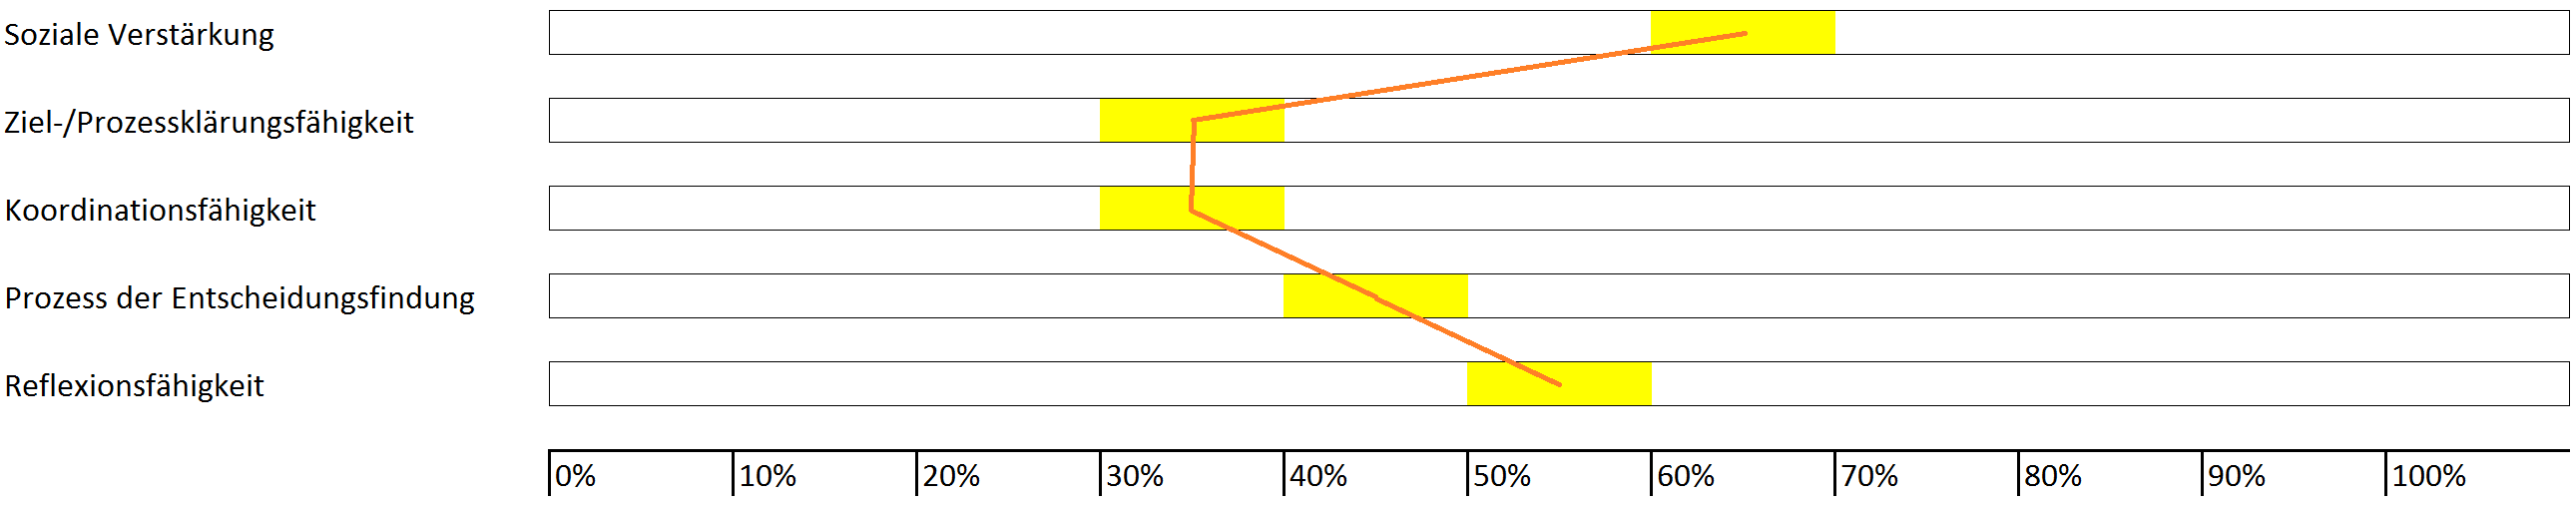
\includegraphics[height=2.8cm]{images/Gruppeneinsch.png}

Am wenigsten ausgeprägt sind die beiden Punkte Prozessklärungsfähigkeit und Koordinationsfähigkeit. Hier hat unser Team das grösste Verbesserungspotenzial. Der Punkt, der am besten bewertet wurde ist die Reflexionsfähigkeit und wir finden, dass wir unser Teamverhalten oft sehr genau analysieren können. 

\begin{comment}
Nach unseren individuell erstellten Selbsteinsch"atzungen, folgen nun die Fremdeinsch"atzungen, welche f"ur
den Vergleich von Selbst- und Fremdbild unabdingbar sind.
Dazu hat jedes Teammitglied seine eigene Form der Bearbeitung gew"ahlt. Dies war einerseits der Selbsteinsch"atzungstest, andererseits wurden anhand von spezifisch beobachteten Situationen eine Teamrollenzuteilung
vorgenommen.
\subsection*{Pascal Horat}

Auch um meine Teamkameraden einzuschätzen habe ich mich des vorher beschriebenen Belbin-Tests bedient. Dies vor allem aus drei Gründen:
\begin{enumerate}
\item Durch die vorgegebene Form ergibt sich meiner Meinung nach eine neutralere Betrachtung der Teamitglieder, da meine Einschätzung nicht nur auf ein bis zwei spezifischen Vorfällen beruht.
\item Durch die vorgegebene Form mit den Aussagen werde ich durch das Verfahren geleitet und muss nicht selber etwas entwickeln.
\item Da für die Bestimmung der Selbst- sowie der Fremdeinschätzung derselbe Test verwendet wurde, können direkte Vergleiche zwischen den Teammitgliedern gemacht werden.
\end{enumerate}

Dies hat für Gerome folgende Resultate hervorgebracht:



Von meinen Teammitgliedern fiel es mir, ohne die Hilfe des Tests, schwieriger, Gerome eine passende Rolle zuzuteilen. Darum hätte ich eine ausgeglichenere Punkteverteilung bei der Auswertung erwartet. Die Rolle des Ausgleichers, bei welcher er am meisten Punkte sammelte, finde ich jedoch passend. Dass sie bei ihm aber so ausgeprägt zum Zuge kommt, hat mich eher überrascht.

Bei Gökhan sieht die Auswertetabelle folgendermassen aus:



Bei ihm habe ich schon im Vornherein erwartet, dass er punktemässig eine Ausgleicher-Rolle erhalten würde. Interessanterweise war diese Rollenzuteilung aber viel ausgeglichener als vorher bei Gerome obwohl ich instinktiv eher das Gegenteil erwartet hätte. 

\subsection*{Steve Gerome Kamga}

Meine beiden Teammitglieder wurden auch von mir mit der Belbin-Methode eingeschätzt und die Ergebnissen werden folgendermassen dargestellt: \\
Nach meiner Einschätzung kam heraus, dass Pascal die nachfolgenden Rollen in einem Team übernehmen könnte:
\begin{enumerate}
\item Koordinator
\item Prozessgestalter
\item Bewerter
\end{enumerate}


Gökhan dagegen ist meiner Meinung nach mehr der:
\begin{enumerate}
\item Bewerter
\item Spezialist
\item Ausgleicher
\end{enumerate}


\subsection*{Gökhan Kaya}

Ich habe meine zwei Teamkollegen folgendermassen eingeschätzt:\\

Pascal war für mich der Koordinator und zwar aus den folgenden erlebten Gründen:
\begin{enumerate} 
\item{Meist sagt Pascal am Anfang der Sitzung was zu tun ist und gibt uns einen kleinen Überblick. Er ist somit sehr gut organisiert.}
\item{Er ist meistens der erste, der sich mit dem Dozenten in Verbindung setzt, wenn etwas noch unklar ist. Die nötigen Informationen leitet er uns anschliessend weiter.}
\item{Bereits bei der ersten Vorlesung ist mir aufgefallen, dass Pascal sich sehr vieles notiert und teilweise nach der Vorlesung ebenfalls mitteilt, was er sich notiert hat.}
\end{enumerate}

Gerome war für mich ganz klar der Vollender. Dies aus den folgenden drei Gründen:
\begin{enumerate} 
\item{Gleich nach der Teambildung konnte Gerome noch nicht auf moodle zugreifen. Er hat sich nach einem Tag bereits sofort gemeldet und mitgeteilt, dass bei ihm nun alles soweit funktioniert. Dies obwohl es nicht nötig gewesen wäre.}
\item{Ebenfalls hat nach der ersten Aufgabenteilung sofort auf WhatsApp geschrieben und uns mitgeteilt, dass er sein Auftrag erledigt hat. Pascal und ich empfanden dies hingegen als nicht nötig.}
\item{Als wir am letzten Tag vor der Abgabe noch bis spät die Lernbilanzen fertig gestellt haben, hat Gerome die ersten zwei Stunden ausschliesslich recherchiert, um das bestmögliche Produkt abzugeben. Dies obwohl wir nur wenig Zeit hatten. Dabei machte es ihm auch nichts aus, bis spät in die Nacht hinein zu arbeiten.}
\end{enumerate}

\end{comment}

%06chapterVergleich.tex

\chapter{Abgeleitete Handlungen}

Nach den obigen Analysen und Diskussionen hat sich unser Team, um die zukünftige Effektivität zu verbessern, auf folgende vier Punkte geeinigt.  

\subsection*{Frühzeitiges Informieren über die Aufträge}

Um zukünftig mehrheitlich agieren zu können und nicht reagieren zu müssen, ist es für unser Team unabdingbar, die Auftragslage so früh und detailliert wie möglich zu klären. Dies beinhaltet unter anderem, dass wir uns über die Aufträge, welche für die übernächste Woche anstehen Infomieren, so dass wir in der letzten Vorlesung vor Abgabe dem Dozenten entsprechende Fragen gestellt werden könnten. 

\subsection*{Mehr sachliche Kritik}  

Nur wenn Regelmössig sachliche Kritik angebracht wird, kann sich unser Team laufend verbessern. Diese sollte als Möglichkeit sich selber zu verbessern zu können angeschaut werden und nicht als persönlicher Angriff aufgefasst werden. 

\subsection*{Bessere Koordination und Aufgabenteilung}

Da das AC-Projekt recht umfangreich sein wird, muss die Aufgabenteilung besser koordiniert werden. Es ist überhaupt nicht effizient alle Arbeiten als Dreierteam zu erledigen. 

\subsection*{Öfters gegenseitiges Nachfragen bei Unklarheiten}

In einem Projekt sollten nach einer gewissen Zeit alle Teammitglieder einen abgeglichenen Wissensstand haben. Aus diesem Grund muss bei Unklarheiten, seien diese administrativer, technischer oder inhaltlicher Natur, sofort bei Teammitgliedern nachgefragt werden.


\nocite{lencioni2010five}
%07chapterZusammenfasssung.tex

\chapter{Todo Liste}

Aus vorangehend aufgelisteten Handlungen sollen nun unter Beachtung der 
SMART-Kriterien (Specific, Measurable, Accepted, Reasonable, Time-bound) 
effektive Massnahmen abgeleitet werden. 

\begin{itemize}

\item Alle Teammitglieder müssen sich ab jetzt schon zwei Wochen vor dem Abgabetermin über die Anstehende Aufträge informiert haben
\item Alle Teammitglieder sollten sich ab jetzt vermehrt sachliche Kritik an ihren Teammitglieder anwenden  
\item Pascal Horat muss viel mehr Aufwand bezüglich der Koordination und Führung \cite{belbin1981management} des Teams betreiben. Dies beinhaltet wöchentliches Anpassen der Detailplanung und regelmässiges Auffordern der Teammitglieder, ihren Arbeitsstand zu vermerken.
\item Steve Gerome Kamga muss zukünftig sich sofort an seine Teammitglieder wenden, falls irgendwelche Unklarheiten bestehen.

\end{itemize}
%08chapterKonsequenzen.tex
\chapter{Protokoll}

Protokoll der Teamsitzung

Datum: 03.04.2017
Ort: HSR Rapperswill

Teilnehmer: Steve Gerome Kamga, Pascal Horat, Gökhan Kaya\\
Sitzungsleiter: Gökhan Kaya

Thema: Teamreview 3

\begin{enumerate}

\item Festlegung des Ablaufs der Sitzung, Eröffnung der Sitzung 

\item  Verteilung der Aufgaben während der Sitzung
\begin{itemize}
\item Gerome: Schreiben der Sitzungsprotokolle
\item Gökhan: Schreiben des TR3
\item Pascal: Erstellen des Diagramms nach Simon und die ToDo Liste
\end{itemize}

\item Besprechung über Selbsteinschätzung zur Teameffektivität
 grafische Darstellung der Selbsteinschätzungen

\item Diskussion über die Gruppeneffektivität\\
Grafische Darstellung der Gruppeneffektivität nach Modell-Simon und Einigung auf eine gemeinsamen Gruppeneischätzung

\item Abgeleitete Handlung
mehr Kritik, Bessere Koordination und Aufgabenteilung, mehr gegenseitiges Nachfragen bei Unklarheiten

\item To Do Liste

Nach SMART-Kriterien wurden neue Regeln definiert und vorgeschlagen
für eine bessere und effizienter Teamarbeit

\item Benötigte Literatur: Simon 2002 

\item Zusammenfassung

\end{enumerate}

Nächste Sitzung: 10.04.2017


% List of figures & glossary
%%%%%%%%%%%%%%%%%%%%%%%%%%%%
%\listoffigures
\printglossary[style=altlist,title=Glossar]

% Bibliography
%%%%%%%%%%%%%%
\bibliographystyle {plain}
\bibliography{index/bibliography}


% Attached sources
%%%%%%%%%%%%%%%%%%
%\input{attachments/attachments}


\end{document}
